
% ============================================================
%  CHAPTER 8 -- Implementation Evidence
% ============================================================
\chapter{Implementation Evidence}
\label{ch:implementation-evidence}

This chapter presents the evidence of the physical and functional
implementation of the gantry crane system. Evidence is provided
for each of the five subsystems, namely EERI I, EERI II, MCTR I,
MCTR II, and REII, followed by evidence of the integrated system.
The purpose is to demonstrate how the design was realised through
fabrication, assembly, electrical integration, and software
implementation, where applicable.

Photographs, engineering drawings, circuit diagrams, software
listings, and other relevant artefacts are included to document
the implementation. Each item of evidence is linked to the
corresponding subsystem or design requirement wherever possible.

\section{EERI I Implementation Evidence}
\label{sec:eeri-i-evidence}

This section documents the implementation of EERI I and provides
evidence of the completed work. The evidence should demonstrate
the physical construction, electrical or mechanical connections,
and other implementation details relevant to the subsystem.

\subsection{Physical Implementation}

Figure~\ref{fig:eeri-i-implementation} presents the implemented
EERI I subsystem.

\begin{figure}[H]
    \centering
    % \includegraphics[width=0.8\textwidth]
    % {img/eeri_i_implementation}
    \caption{Implemented EERI I subsystem.}
    \label{fig:eeri-i-implementation}
\end{figure}

The figure should identify the principal components and show
how they are assembled or connected. Any differences between
the final implementation and the original design should be
documented and justified.

\subsection{Supporting Design Evidence}

Supporting evidence may include circuit diagrams, CAD drawings,
schematics, component specifications, fabrication photographs,
or relevant software listings, depending on the nature of EERI I.

\begin{figure}[H]
    \centering
    % \includegraphics[width=0.8\textwidth]
    % {img/eeri_i_design}
    \caption{Design documentation for EERI I.}
    \label{fig:eeri-i-design}
\end{figure}

\section{EERI II Implementation Evidence}
\label{sec:eeri-ii-evidence}

This section presents the evidence demonstrating the
implementation of EERI II.

\subsection{Physical Implementation}

Figure~\ref{fig:eeri-ii-implementation} shows the completed
EERI II subsystem.

\begin{figure}[H]
    \centering
    % \includegraphics[width=0.8\textwidth]
    % {img/eeri_ii_implementation}
    \caption{Implemented EERI II subsystem.}
    \label{fig:eeri-ii-implementation}
\end{figure}

The implementation evidence should identify the principal
components, their arrangement, and their connection to the
relevant parts of the gantry crane system.

\subsection{Supporting Design Evidence}

The final implementation should be supported by relevant
engineering drawings, electrical schematics, component
documentation, or other records showing how the design
was realised.

\begin{figure}[H]
    \centering
    % \includegraphics[width=0.8\textwidth]
    % {img/eeri_ii_design}
    \caption{Design documentation for EERI II.}
    \label{fig:eeri-ii-design}
\end{figure}

\section{MCTR I Implementation Evidence}
\label{sec:mctr-i-evidence}

This section documents the construction and assembly of MCTR I.
Evidence should demonstrate the implemented components and
their relationship to the subsystem's intended function.

\subsection{Fabrication and Assembly}

Figure~\ref{fig:mctr-i-implementation} presents the implemented
MCTR I subsystem.

\begin{figure}[H]
    \centering
    % \includegraphics[width=0.8\textwidth]
    % {img/mctr_i_implementation}
    \caption{Implemented MCTR I subsystem.}
    \label{fig:mctr-i-implementation}
\end{figure}

Where applicable, the evidence should show the materials used,
fabrication methods, fasteners, joints, alignment, and the
assembly of the relevant components. Any significant deviations
from the design drawings should be explained.

\subsection{Engineering Drawings and Supporting Evidence}

The implementation should be supported by the relevant
mechanical drawings, CAD models, dimensions, and photographs
of the fabrication or assembly process, where available.

\begin{figure}[H]
    \centering
    % \includegraphics[width=0.8\textwidth]
    % {img/mctr_i_design}
    \caption{Engineering drawing or CAD representation of MCTR I.}
    \label{fig:mctr-i-design}
\end{figure}

\section{MCTR II Implementation Evidence}
\label{sec:mctr-ii-evidence}

This section presents evidence of the implementation of MCTR II,
including its construction, assembly, and integration with
the relevant parts of the gantry crane up to date at the time of this reports publication.

\subsection{Fabrication and Assembly}

Figure~\ref{fig:mctr-ii-implementation} shows the components up to dat 

\begin{figure}[H]
    \centering
     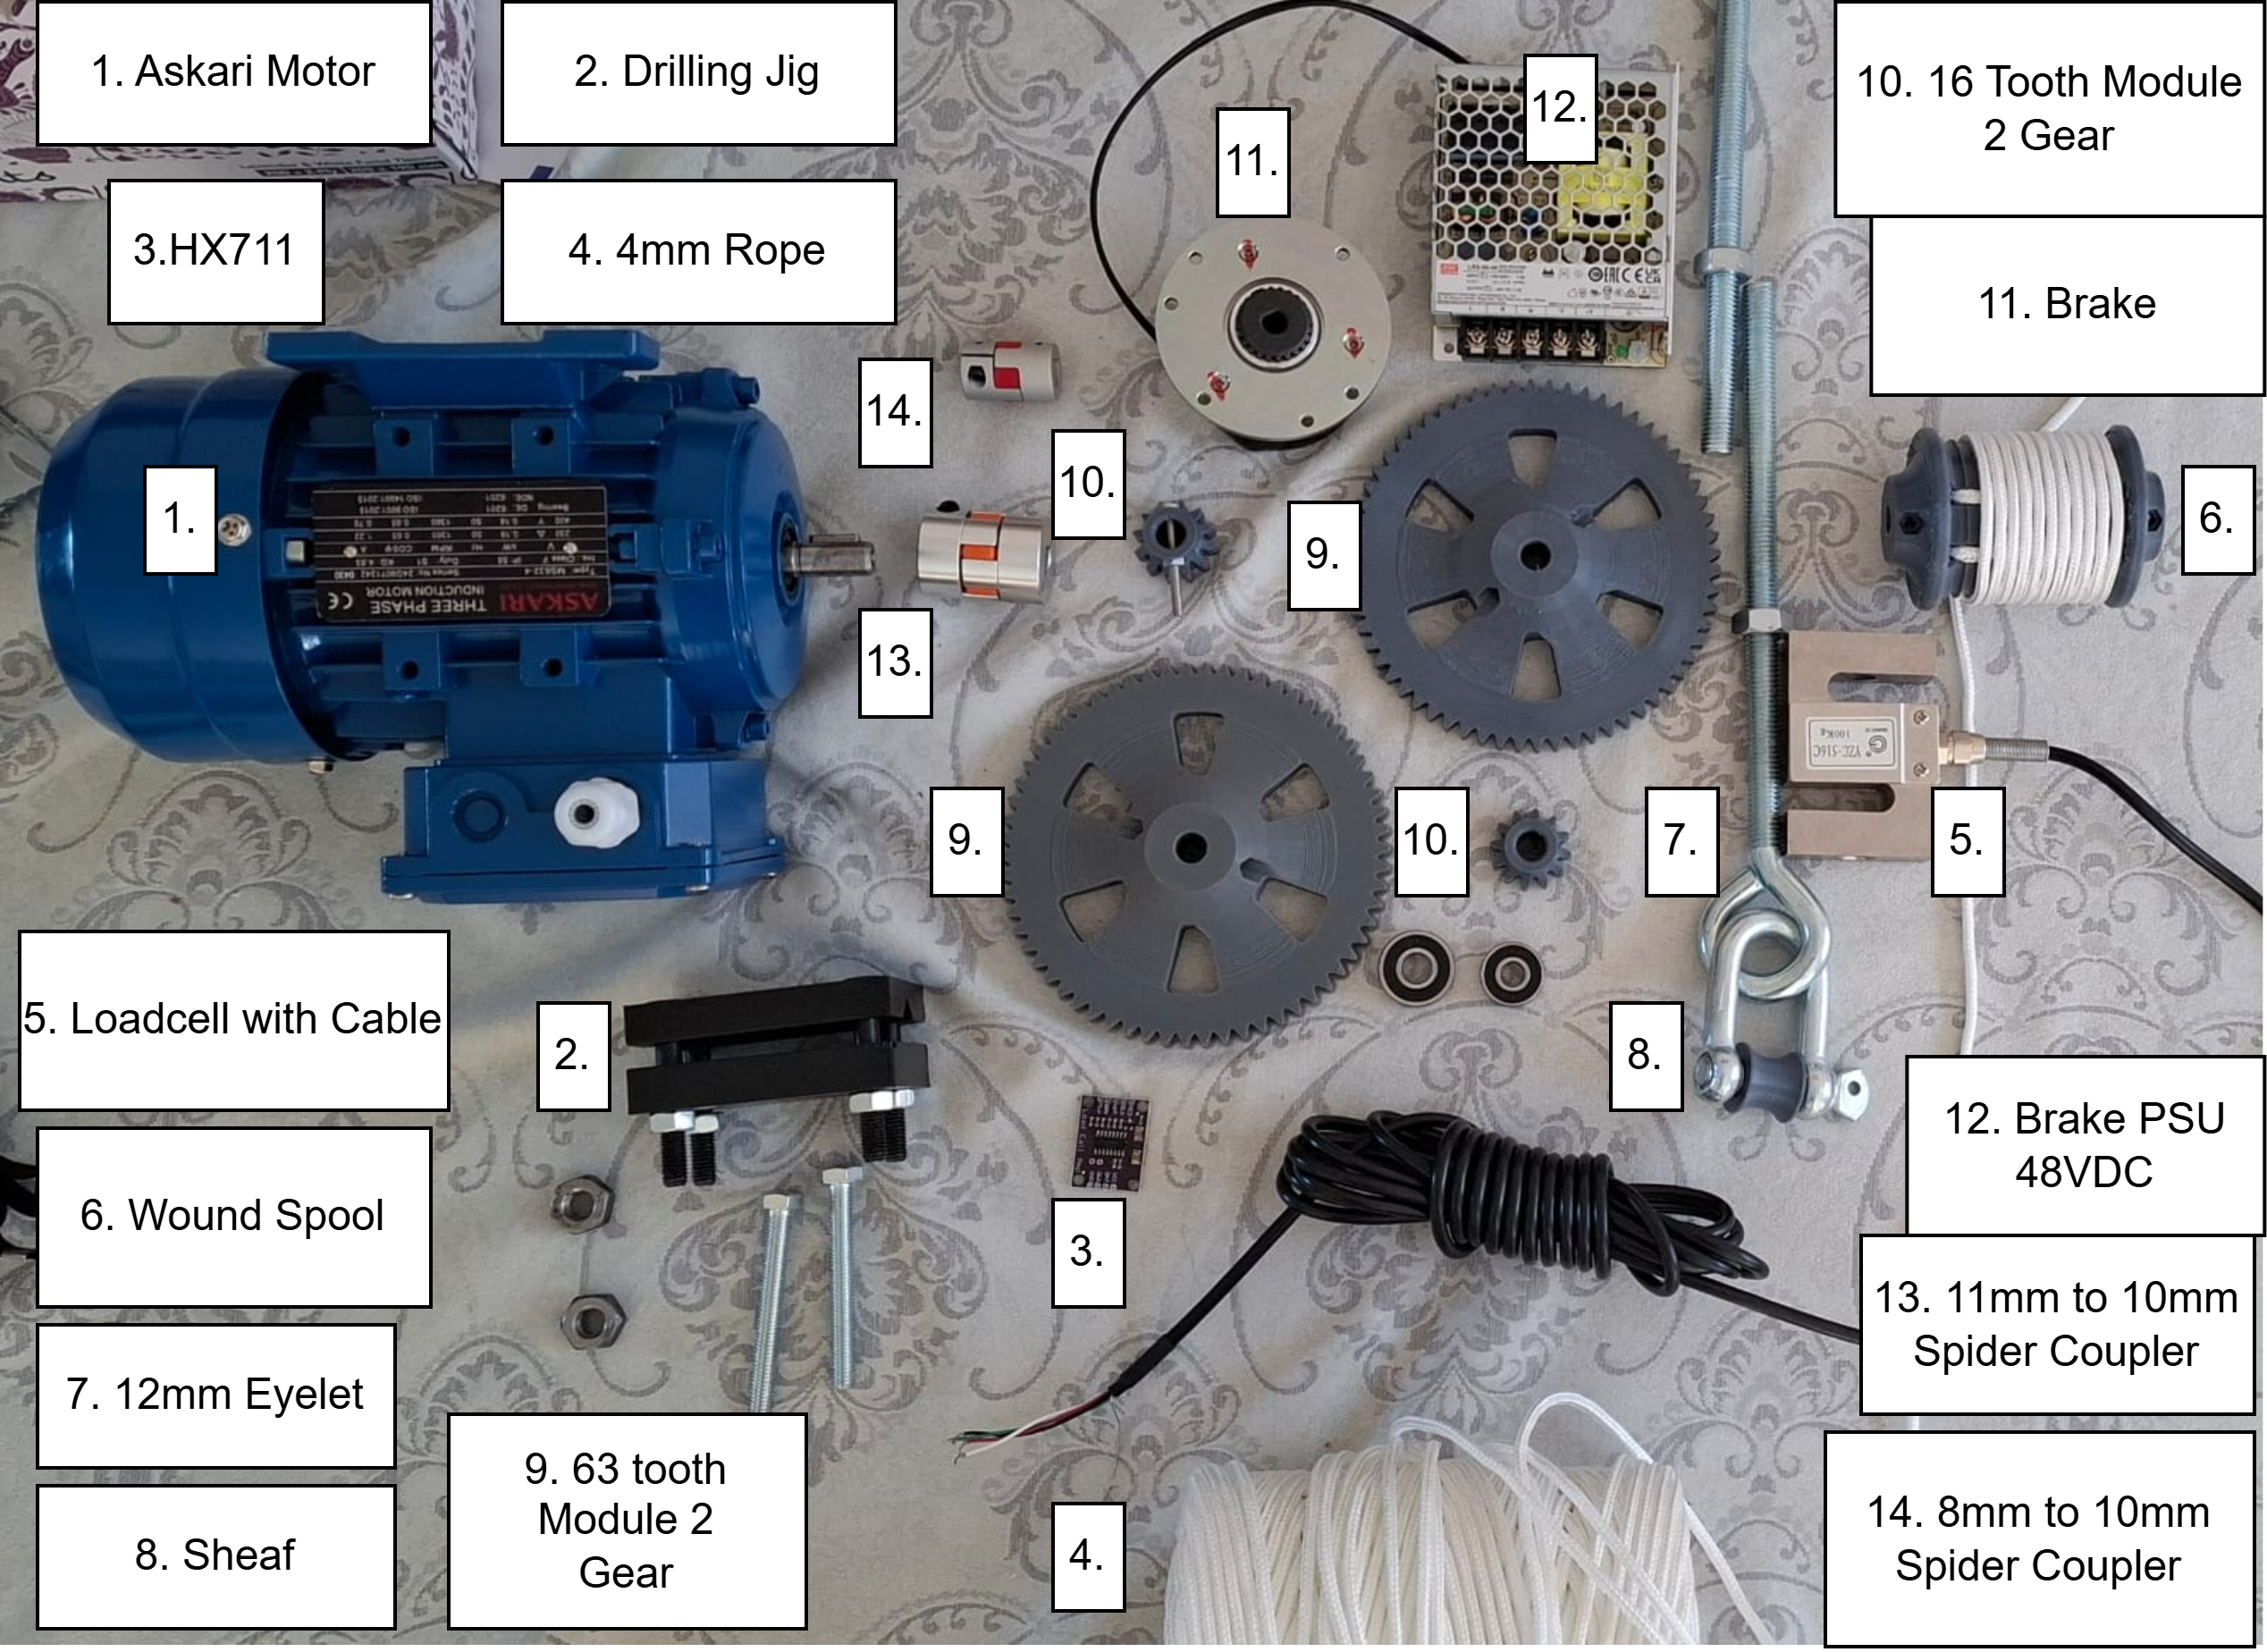
\includegraphics[width=0.8\textwidth]{figures/Fig_Components_and_Parts_MCTRII.png}
    \caption{All Components for MCTR II Up to Date of Report Publication.}
    \label{fig:mctr-ii-implementation}
\end{figure}

The main components in this iamge are those that have been acquired up to date. The mild steel rods had been acquired within the week of writing this report and thus still need to be processed. In the image each of the components are numbered and named with the most prominent designed components the 4 gears to be used in the 2 stages in that configuration, with the gear at ~10. showing the method that will be used to fasten it to the shaft with a throughhole bolt and nut. The other gears will be fastened likewise. The eyebolts will be cut to size and used to fasten to MCTR I

\subsection{Engineering Drawings and Supporting Evidence}

Supporting evidence may include CAD drawings, component
specifications, assembly photographs, and other records that
demonstrate how MCTR II was constructed.

\begin{figure}[H]
    \centering
    % \includegraphics[width=0.8\textwidth]
    % {img/mctr_ii_design}
    \caption{Engineering drawing or CAD representation of MCTR II.}
    \label{fig:mctr-ii-design}
\end{figure}

\section{REII Implementation Evidence}
\label{sec:reii-evidence}
\label{sec:sw-impl}

This section presents the available evidence from earlier
REII hardware testing and software development.
Implementation of the final ESP32-S3 crane system remains
incomplete.

\subsection{Physical Implementation}

Figure~\ref{fig:reii-implementation} shows the earlier
radio bench comprising two ESP32 boards and two nRF24
modules. Later bench firmware generated physical PWM
outputs while motion and sensor readings were simulated.
The current controller is the university-supplied
ESP32-S3 board, which still requires firmware migration
and crane integration.

\begin{figure}[H]
    \centering
    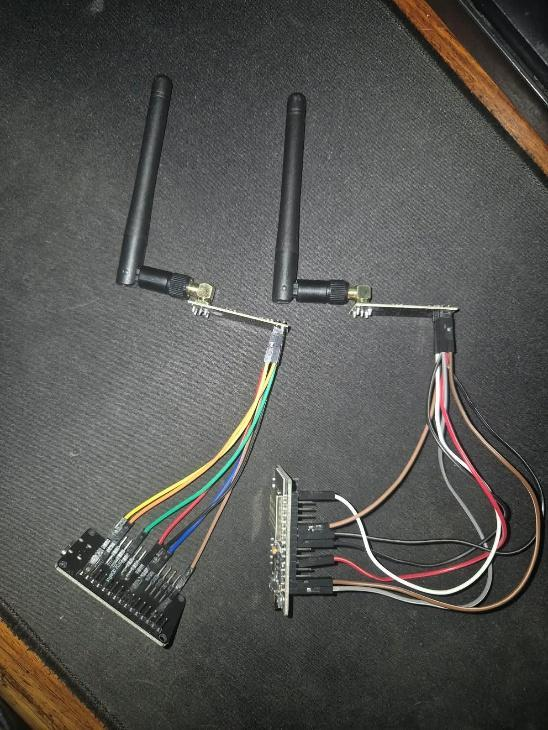
\includegraphics[width=0.32\textwidth]
        {figures/Figure_8_9_Radio_Assembly.jpg}
    \caption{Earlier two-ESP32/nRF24 radio bench assembly.}
    \label{fig:reii-implementation}
\end{figure}

\subsection{Supporting Design Evidence}

Figure~\ref{fig:reii-design} shows the proposed software
arrangement linking the Python dashboard, STM32 ground
station and ESP32-S3 controller. The existing dashboard,
STM32 bridge and earlier ESP32 controller software would
provide the basis for this implementation.

The Excel workbook records the earlier radio measurements.
\cite{reii_measurements2026}
Migration to the ESP32-S3 and integrated testing of the
sensors, brake and complete crane remain outstanding.

\begin{figure}[H]
    \centering
    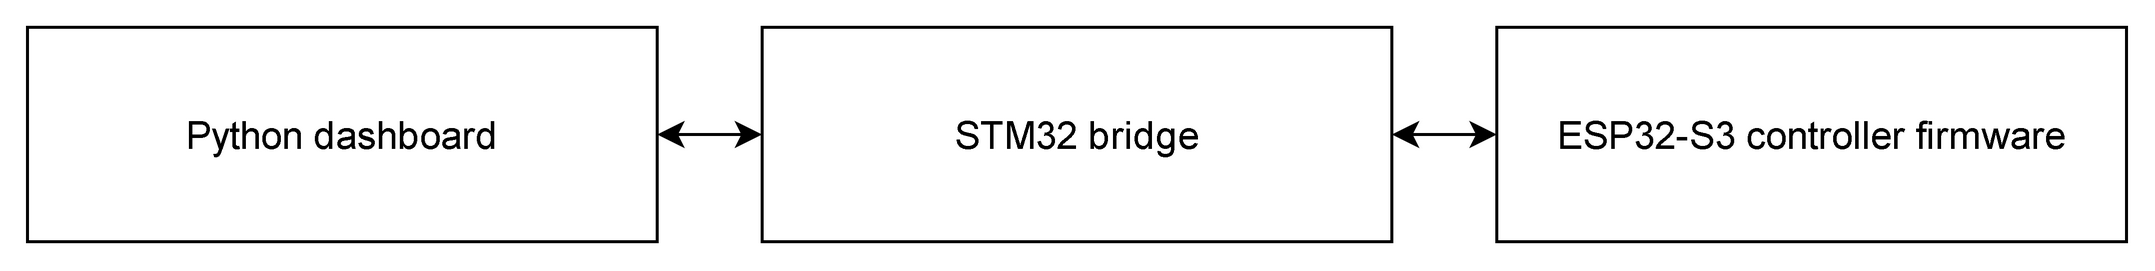
\includegraphics[width=0.95\textwidth]
        {figures/Figure_8_10_Software_Sources.png}
    \caption{Proposed REII software arrangement.
        ESP32-S3 migration remains incomplete.}
    \label{fig:reii-design}
\end{figure}

\section{Integrated System Implementation}
\label{sec:integrated-system-evidence}

This section demonstrates how the five subsystems were assembled
and integrated into the complete gantry crane system. The evidence
should show the overall arrangement and the interfaces between
the subsystems.

\subsection{Final Assembly}

Figure~\ref{fig:integrated-system-evidence} presents the assembled
gantry crane.

\begin{figure}[H]
    \centering
    % \includegraphics[width=0.85\textwidth]
    % {img/integrated_system}
    \caption{Completed gantry crane system.}
    \label{fig:integrated-system-evidence}
\end{figure}

The figure should demonstrate the overall arrangement of the
implemented system and identify the locations of EERI I, EERI II,
MCTR I, MCTR II, and REII. Multiple views may be provided where
necessary to show interfaces that cannot be seen in a single
photograph.

\subsection{Subsystem Interfaces}

The subsystem interfaces shall be documented using appropriate
photographs, assembly drawings, wiring diagrams, or interface
schematics. These records should show how the subsystems are
physically and functionally connected.

\begin{figure}[H]
    \centering
    % \includegraphics[width=0.85\textwidth]
    % {img/system_interfaces}
    \caption{Interfaces between the implemented subsystems.}
    \label{fig:system-interfaces}
\end{figure}

The evidence should be consistent with the subsystem interface
matrix in Chapter~\ref{ch:system-performance}, or the relevant
chapter in which the interface analysis is presented. Any
modifications made during integration should be documented.

\section{Implementation Evidence Summary}
\label{sec:implementation-evidence-summary}

Table~\ref{tab:implementation-evidence-summary} summarises the
evidence provided for each subsystem and the integrated system.

\begin{table}[H]
    \centering
    \caption{Summary of implementation evidence.}
    \label{tab:implementation-evidence-summary}
    \renewcommand{\arraystretch}{1.4}
    \begin{tabularx}{\textwidth}{|X|X|X|}
        \hline
        \textbf{Subsystem} &
        \textbf{Evidence provided} &
        \textbf{Implementation status} \\
        \hline
        EERI I &
        [Photographs, drawings, schematics, or other evidence] &
        [Completed / Partial / Not implemented] \\
        \hline
        EERI II &
        [Photographs, drawings, schematics, or other evidence] &
        [Completed / Partial / Not implemented] \\
        \hline
        MCTR I &
        [Photographs, CAD drawings, assembly records, or other evidence] &
        [Completed / Partial / Not implemented] \\
        \hline
        MCTR II &
        [Photographs, CAD drawings, assembly records, or other evidence] &
        [Completed / Partial / Not implemented] \\
        \hline
        REII &
        [Photographs, drawings, schematics, or other evidence] &
        [Completed / Partial / Not implemented] \\
        \hline
        Integrated system &
        [Overall assembly photographs and interface evidence] &
        [Completed / Partial / Not implemented] \\
        \hline
    \end{tabularx}
\end{table}

The evidence presented in this chapter documents the extent to
which the design has been implemented. The implementation records
provide a basis for interpreting the performance results presented
in Chapter~\ref{ch:system-performance}. Evidence of physical
construction alone does not establish that the system meets its
performance requirements; this must be demonstrated by the
relevant verification and validation results.
